%\documentclass[mathserif]{beamer}
\documentclass[handout]{beamer}
%\usetheme{Goettingen}
\usetheme{Warsaw}
%\usetheme{Singapore}
%\usetheme{Frankfurt}
%\usetheme{Copenhagen}
%\usetheme{Szeged}
%\usetheme{Montpellier}
%\usetheme{CambridgeUS}
%\usecolortheme{}
%\setbeamercovered{transparent}
\usepackage[english, activeacute]{babel}
\usepackage[utf8]{inputenc}
\usepackage{amsmath, amssymb}
\usepackage{dsfont}
\usepackage{graphics}
\usepackage{cases}
\usepackage{graphicx}
\usepackage{pgf}
\usepackage{epsfig}
\usepackage{amssymb}
\usepackage{multirow}	
\usepackage{amstext}
\usepackage[ruled,vlined,lined]{algorithm2e}
\usepackage{amsmath}
\usepackage{epic}
\usepackage{epsfig}
\usepackage{fontenc}
\usepackage{framed,color}
\usepackage{palatino, url, multicol}
\usepackage{listings}
%\algsetup{indent=2em}


\vspace{-0.5cm}
\title{Introduction to R}
\vspace{-0.5cm}
\author[Felipe Bravo Márquez]{\footnotesize
%\author{\footnotesize  
 \textcolor[rgb]{0.00,0.00,1.00}{Felipe José Bravo Márquez}} 


\date{ \today }


\begin{document}
\begin{frame}
\titlepage


\end{frame}


%%%%%%%%%%%%%%%%%%%%%%%%%%%


\section{Introduction}




\begin{frame}{The R project for computational statistics}
\begin{figure}[h!]
	\centering
	
\includegraphics[scale=0.6]{pics/Rlogo.png}
\end{figure}
\scriptsize{
\begin{itemize}
 \item R is a free statistical programming environment: \url{http://www.r-project.org/}
 \item It allows to manipulate and store data in an effective way.
 \item R is a complete programming language: variables, loops, conditions, functions.
 \item It provides many libraries that implement pretty much any statistical method.
 \item These libraries together with their dependencies are organized in a repository called \textbf{CRAN}: \url{http://cran.r-project.org/}



\end{itemize}

}



\end{frame}


\begin{frame}{Why use R?}


\scriptsize{
\begin{itemize}
 \item R is free software unlike Matlab, SPSS, STATA.
 \item It is available for many operating systems: Windows, MAC OS X, Linux.
 \item As of 2013 \textbf{KDnuggets} survey showed R as the preferred programming language for performing data analysis, data mining and data science.
 \item \url{http://www.kdnuggets.com/2013/08/languages-for-analytics-data-mining-data-science.html}
 \item Today Python has become a very strong competitor.


\end{itemize}

}

\begin{figure}[h!]
	\centering
	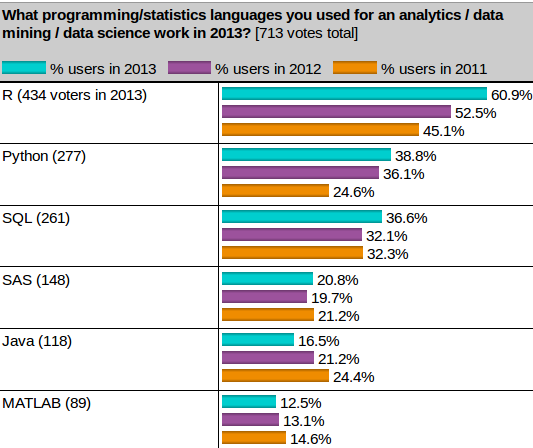
\includegraphics[scale=0.3]{pics/rpoll.png}
\end{figure}


\end{frame}

\begin{frame}{RStudio}
\scriptsize{
\begin{itemize}
  \item R works through the command line.
 \item To work in a more friendly environment we will use RStudio.
 \item It is also free and can be downloaded for different operating systems at this link: \url{https://www.rstudio.com/products/rstudio/download/}
\end{itemize}

} 

\begin{figure}[h!]
	\centering
	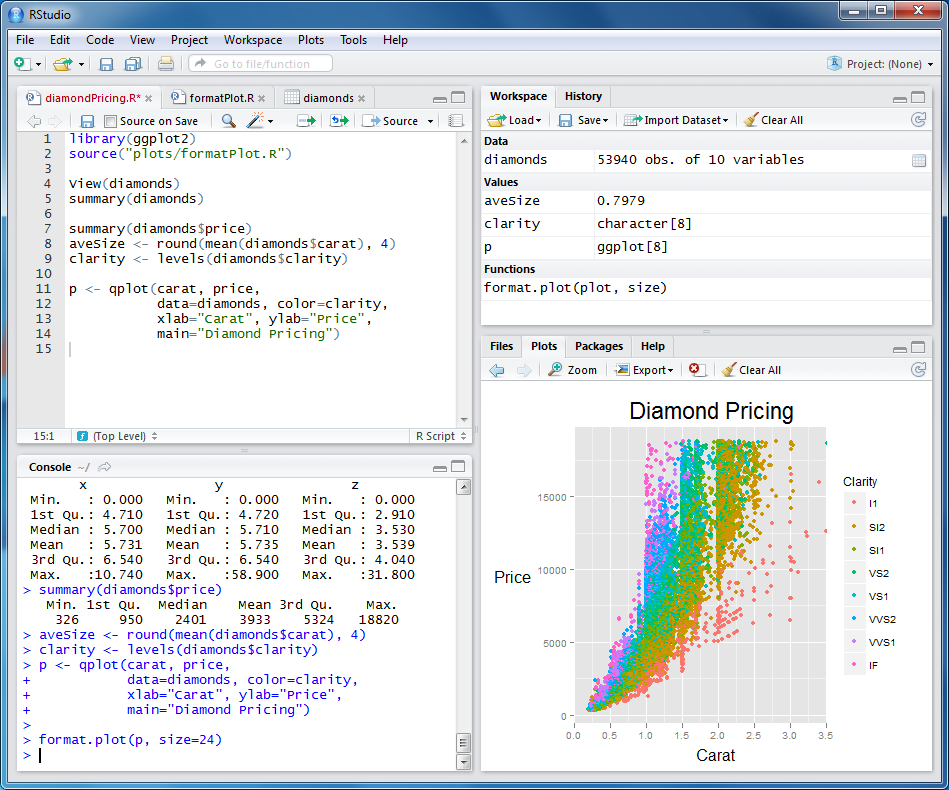
\includegraphics[scale=0.2]{pics/rstudio.png}
\end{figure}

 
\end{frame}


\section{R basic commands}

\begin{frame}[fragile]{R as a calculator}
\begin{verbatim}
> 4*5
[1] 20
> 2^3
[1] 8
> exp(-5)
[1] 0.006737947
> log(4)
[1] 1.386294
\end{verbatim}

\footnotemark{The following slides are based on \cite{venables2009introduction}}
 
\end{frame}




\begin{frame}[fragile]{Declaring Variables}
\scriptsize{
\begin{itemize}
 \item Variables can be assigned using \verb+<-+ , \verb+=+ or the function \verb+assign+.
 
  \begin{verbatim}
a<-1
b=3
assign("three",3)
d<-a+b
ver<-T # equivalent to TRUE
word<-"hello"
\end{verbatim}
 
 \item By convention we use the first form (\verb+<-+).
 
\item Variables can be of class \textbf{numeric}, \textbf{factor}, \textbf{character}, \textbf{logical}, among others.
 
\item To see the type of a variable we use the command \verb+class+.
 \begin{verbatim}
  > class(a) 
[1] "numeric"
> class(ver)
[1] "logical"
> class(word)
[1] "character"
 \end{verbatim}

 
 
\end{itemize}

}


\end{frame}


\begin{frame}[fragile]{Functions}
\scriptsize{
\begin{itemize}
 \item Functions are declared as variables and are created with the expression \textbf{function}:

\begin{verbatim}
my.sum<-function(a=2,b=1){
  return(a+b);
}

fac<-function(n){
  ifelse(n==1,return(1),return(n*fac(n-1)))    
}

\end{verbatim}

\item Function parameters can be declared with a specific value to be used as default values when we do not provide values for those parameters:
\begin{verbatim}
> my.sum(3,4)
[1] 7
> my.sum()
[1] 3 
\end{verbatim}

\item The functions are of the type \textbf{function}:
\begin{verbatim}
> class(my.sum)
[1] "function" 
\end{verbatim}


\end{itemize}


 
} 
\end{frame}

\begin{frame}[fragile]{Help and Workspace}
\scriptsize{
\begin{itemize}
 \item To read documentation about a function we use either \textbf{help} or \textbf{?}:
\begin{verbatim}
help(ls)
?ls
#for a particular command
help("for")
\end{verbatim}

\item All variables are stored in my \textbf{workspace} environment. To list them we use the command \textbf{objects} or \textbf{ls}. To delete a variable we use \textbf{rm}:

\begin{verbatim}
objects()
ls()
rm(a)
#to delete them all
rm(list=ls())
 
\end{verbatim}


\item We can save all my workspace variables in a file and then retrieve my work in a future session:
\begin{verbatim}
save.image("myworkspace.RData")
# we can load it in a new session
load("myworkspace.RData")
 
\end{verbatim}


 
 
 
 \end{itemize}



}
 
 
\end{frame}

\begin{frame}[fragile]{Vectors}
\scriptsize{
\begin{itemize}
 \item To work with collections of elements we declare \textbf{vectors} which are constructed with the command \textbf{c}:
 \begin{verbatim}
ages<-c(21,33,12,34,23,70,90,80,7,29,14,2,
          88,11,55,24,13,11,56,28,33)
 \end{verbatim}
 \item To get the length of a vector we use the command \textbf{length}, then to get the sum of all elements we use \textbf{sum}:
 \begin{verbatim}
> a.sum<-sum(ages)
> a.length<-length(ages)
> a.sum
[1] 734
> a.length
[1] 21
 \end{verbatim}
 
\item If we operate a vector by a scalar this value is recycled for all elements of the vector:
 \begin{verbatim}
> numbers<-c(1,2,3)
> numbers+3
[1] 4 5 6
> numbers*5
[1]  5 10 15
 \end{verbatim}
\end{itemize}




}
 
 
\end{frame}

\begin{frame}[fragile]{Vectors (2)}
\scriptsize{
\begin{itemize}
 \item Calculate the mean and variance of the vector ages using the commands \textbf{sum} and \textbf{length} based on the following equations:
 \begin{equation}
  \text{mean}(\text{ages})=\frac{\sum_{i=1}^n\text{ages}_{i}}{n}
 \end{equation}
 
 \begin{equation}
 \text{variance}(\text{ages})=\frac{\sum_{i=1}^n(\text{ages}_{i}-\text{media}(\text{ages}))^2 }{n-1} 
 \end{equation}

 
\end{itemize}



}

 
\end{frame}



\begin{frame}[fragile]{Vectors (3)}
\scriptsize{
\begin{itemize}
 \item Answer:
 \begin{verbatim}
> a.mean<-sum(ages)/length(ages)
> a.mean
[1] 34.95238
> a.var<-sum((ages-a.mean)^2)/(length(ages)-1)
> a.var
[1] 747.9476
 \end{verbatim}
 
 \item R provides \textbf{mean} and \textbf{var} functions:
 \begin{verbatim}
> mean(ages)
[1] 34.95238
> var(ages)
[1] 747.9476

 \end{verbatim}
 
\end{itemize}



}

 
\end{frame}
 
 
\begin{frame}[fragile]{Vectors (4)}
\scriptsize{
\begin{itemize}
 
\item When we construct vectors with elements of different types, R converts them all to a single type:
\begin{verbatim}
> c("hello",2,T)
[1] "hello" "2"    "TRUE"
> c(TRUE,FALSE,500)
[1]   1   0 500 
\end{verbatim}

 \item The elements of a vector can be declared with names and then retrieved with the \textbf{names} command:
\begin{verbatim}
> grades<-c(Juan=4.5,Luis=6.2,Romina=3.9,Felipe=2.8,Mariana=6.7)
> names(grades)
[1] "Juan"    "Luis"    "Romina"  "Felipe"  "Mariana"
 
\end{verbatim}
\item We can sort a vector using the \textbf{sort} command:
\begin{verbatim}
> names(sort(x=grades,decreasing=T))
[1] "Mariana" "Luis"    "Juan"    "Romina"  "Felipe" 
\end{verbatim}

\end{itemize}



}
\end{frame}

\begin{frame}[fragile]{Vector Access}
\scriptsize{
\begin{itemize}

 \item R allows access to the elements of a vector by means of numerical indexes \verb+[i]+: 
\begin{verbatim}
> grades[1] # first element
Juan 
 4.5
\end{verbatim}

\item The index can be another numeric vector to access more than one element:
\begin{verbatim}
> grades[c(1,5)] # first and fifth element
   Juan Mariana 
    4.5     6.7 
\end{verbatim}

\item If we want to omit any element we use negative indexes:
\begin{verbatim}
> grades[-2] # All but the second one
   Juan  Romina  Felipe Mariana 
    4.5     3.9     2.8     6.7 
\end{verbatim}

\item The elements can also be accessed by their names:
\begin{verbatim}
> grades[c("Juan","Mariana")] # Only Juan and Mariana
   Juan Mariana 
    4.5     6.7 
\end{verbatim}



\end{itemize}

 

 }
\end{frame}


\begin{frame}[fragile]{Operating Vectors}
\scriptsize{
\begin{itemize}
 \item We saw earlier that if we operate a scalar by a vector, the scalar applies to all the elements of the vector.
 \item If we now have two vectors of the same length and operate on them, the operation is done element by element (element-wise):
\begin{verbatim}
a<-c(1,2)
b<-c(3,4)
> a+b
[1] 4 6
> a*b
[1] 3 8
\end{verbatim}

\end{itemize}
 }
\end{frame}



\begin{frame}[fragile]{Operating Vectors (2)}
\scriptsize{
\begin{itemize}
\item If the vectors are of different lengths, the smaller one recycles its elements:
\begin{verbatim}
> d<-c(4,5,6,9)
> a+d
[1]  5  7  7 11
> c(a,a)+d
[1]  5  7  7 11
\end{verbatim}

\item If the length of the longest is not a multiple of the length of the shortest, we get a warning:
\begin{verbatim}
> c(1,2)+c(-9,2,3)
[1] -8  4  4
Warning message:
In c(1, 2) + c(-9, 2, 3) :
  longer object length is not a multiple of shorter object length 
\end{verbatim}
 
\end{itemize}
 }
\end{frame}



\begin{frame}[fragile]{Comparing Vectors}
\scriptsize{
\begin{itemize}
 \item R supports the comparison operators for numeric variables:\verb+ >,<, ==, <=, >=, !=+ in addition to \verb+& |+ as well as the operators \textbf{and} and \textbf{or} for logical variables:
\begin{verbatim}
> younger<-ages<18
> younger
 [1] FALSE FALSE  TRUE FALSE FALSE FALSE FALSE FALSE  TRUE FALSE  TRUE  TRUE FALSE  TRUE FALSE FALSE
[17]  TRUE  TRUE FALSE FALSE FALSE
\end{verbatim}
\item If we give a vector an index of logical variables we retrieve the values where the index takes the true value: 
\begin{verbatim}
> ages[younger] 
[1] 12  7 14  2 11 13 11
\end{verbatim}

\item Exercise: calculate the average age of the elements older or equal to 18 years old.
\begin{verbatim}
mean(ages[ages>=18]) 
\end{verbatim}

 
\end{itemize}



}
\end{frame}

\begin{frame}[fragile]{Null Values}
\scriptsize{
\begin{itemize}
\item In R, missing values are written as \verb+NA+. It is common that they appear when we read data from a database. Some functions do not accept null values so they must be taken into account.
\begin{verbatim}
> missing_vector<-c(12,15,NA)
> missing_vector
[1] 12 15 NA
\end{verbatim}

\item To check if a variable is null we use the command \verb+is.na+:
\begin{verbatim}
> missing_vector[!is.na(missing_vector)]
[1] 12 15 
\end{verbatim}



\end{itemize}

 }
 
 
\end{frame}




\begin{frame}[fragile]{Sequences}
 \scriptsize{
 
 \begin{itemize}
  \item To create a vector consisting of a sequence of numbers we use the command \textbf{seq}:
 
 \begin{verbatim}
> my_pairs<-seq(from=2,to=20,by=2)
> mult_four<-seq(from=4,by=4,length=100)
> pares
 [1]  2  4  6  8 10 12 14 16 18 20
 \end{verbatim} 
 \item It can also be created using the operator (\verb+:+):
 \begin{verbatim}
> 1:10
 [1]  1  2  3  4  5  6  7  8  9 10 
> seq(1,10,1)
 [1]  1  2  3  4  5  6  7  8  9 10
 \end{verbatim} 
 \end{itemize}
 
 }
\end{frame}

\begin{frame}[fragile]{Repetitions}
\scriptsize{
\begin{itemize}
 \item To create vectors that repeat a value or another vector multiple times we use the command \textbf{rep}. The first value is the object to repeat and the second is the number of repetitions:
 \begin{verbatim}
> rep(10,3)
[1] 10 10 10
> rep(c("hello", "bye"),4)
[1] "hello" "bye" "hello" "bye" "hello" "bye"
"hello" "bye" "hello" "bye"
 \end{verbatim}
  \item Problem: Create a sequence that repeats 3 times the first 4 multiples of 7.
 \begin{verbatim}
> rep(seq(from=7,by=7,length=4),3)
 [1]  7 14 21 28  7 14 21 28  7 14 21 28
\end{verbatim}
 
 
\end{itemize}
 
 
 
} 
\end{frame}

\begin{frame}[fragile]{Random vector generation}
\scriptsize{
\begin{itemize}
 \item To perform experiments or simulate phenomena of known behavior it is very useful to generate random vectors.
 \item  If we want uniformly distributed numbers between a maximum and a minimum we use \textbf{runif}:
 \begin{verbatim}
> runif(n=5, min = 1, max = 10)
[1] 5.058862 1.737830 9.450956 9.149376 2.652774
 \end{verbatim}
 \item  If we want numbers centered on a mean $\mu$ with a standard deviation $\sigma$, we use a normal distribution with the command \textbf{rnorm} where we know that $68\%$  of the observations will be within the range $\mu\pm\sigma$, $95\%$ in $\mu\pm2\sigma$ and $99.7\%$ in $\mu\pm3\sigma$:
 
 \begin{verbatim}
> rnorm(n=5, mean = 10, sd = 4)
[1] 12.081286  2.636001 16.001953  0.120463  6.211835
 \end{verbatim}
 
\end{itemize}

}
\end{frame}

\begin{frame}[fragile]{Random Vector Generation (2)}
\scriptsize{
\begin{itemize}
 \item When we want to model the number of arrivals per unit of time to simulate queuing models, we use the \textbf{Poisson} distribution with \textbf{rpos}. The parameter $\lambda$ tells us the average number of arrivals per time period
 \begin{verbatim}
> rpois(n=10, lambda = 3)
 [1] 1 3 8 6 1 1 6 3 4 7
 \end{verbatim}

 \item The binomial distribution can be used to represent experiments in which $k$ independent trials of a coin tossing Bernoulli experiment are performed. The probability of success (e.g., getting a head) in each trial is $p$.  We can simulate the number of hits obtained for $n$ different Binomial experiments with the command \textbf{rbinom} ($k$ is named as ``size'').
\begin{verbatim}
> rbinom(n=10,size=2,prob=0.5)
 [1] 0 1 2 1 1 0 2 0 0 1
> rbinom(n=10,size=2,prob=0.7)
 [1] 1 2 2 1 0 1 2 2 2 2
> rbinom(n=10,size=2,prob=0.2)
 [1] 0 0 0 0 1 0 1 0 1 0 
\end{verbatim}

 
 
\end{itemize}


}
\end{frame}


\begin{frame}[fragile]{Categorical Variables or Factors}
\scriptsize{
\begin{itemize}
 \item In addition to numerical or logical variables, it is possible to work with categorical variables. E.g.: color, gender, social class.
 \item They are created with the command \textbf{factor} and the possible values of the variable are stored in the attribute \textbf{levels}.
\begin{verbatim}
> people<-factor(c("Hombre","Mujer","Mujer","Mujer","Hombre"))
> people
[1] Hombre Mujer  Mujer  Mujer  Hombre
Levels: Hombre Mujer
> class(people)
[1] "factor"
> levels(people)
[1] "Hombre" "Mujer" 
#We can rename the levels
> levels(people)<-c("Man","Woman")
> people
[1] Man   Woman Woman Woman Man  
Levels: Man Woman
\end{verbatim}
 
\end{itemize}

}
\end{frame}


\begin{frame}[fragile]{Aggregating variables by category with \textbf{tapply}}
\scriptsize{
\begin{itemize}
 \item If we have a numeric vector and a categorical vector of the same length we can apply the aggregation function \textbf{tapply}.
 \item Example: let's create a category for the vector ``ages'' with levels \emph{child}, \emph{adolescent}, \emph{adult}:
 \begin{verbatim}
categ_ages<-ifelse(ages<12,"child",
                      ifelse(ages<18,"adolescent","adult"))
class(categ_ages)
[1] "character"
#We convert variables to factor with as.factor
categ_ages<-as.factor(categ_ages)
 \end{verbatim}

 \item Now, we can count the number of people per category, and calculate the mean and standard deviation for each group:
\begin{verbatim}
> tapply(ages,categ_ages,length)
adolescent      adult      child 
         3         14          4 
> tapply(ages,categ_ages,mean)
adolescent      adult      child 
  13.00000   47.42857    7.75000 
> tapply(ages,categ_ages,sd)
adolescent      adult      child 
  1.000000  25.294312   4.272002  
\end{verbatim}

 
\end{itemize}



}
\end{frame}


\begin{frame}[fragile]{Strings}
\scriptsize{
 \begin{itemize}
  \item We can print a string using the command \textbf{cat}:
\begin{verbatim}
> greeting<-"Hello World"
> cat(greeting)
Hello World
\end{verbatim}

\item To concatenate two strings we can use the command \textbf{paste}:
\begin{verbatim}
> paste("Hello","Bye",sep="-")
[1] "Hola-Bye"
> paste("person",1:4, sep="")
[1] "person1" "person2" "person3" "person4"
> paste(greeting,1:3, sep=" ")
[1] "Hello World 1" "Hello World 2" "Hello World 3"
\end{verbatim}

\item To extract substrings we use the command \textbf{substr}:
\begin{verbatim}
> substr(greeting,1,4)
[1] "Hell" 
\end{verbatim}

\item There is a vector called \textbf{letters} that has all the letters of the alphabet. It is useful for naming variables:
\begin{verbatim}
> letters[1:4]
[1] "a" "b" "c" "d" 
\end{verbatim}


 \end{itemize}

 }
\end{frame}


\begin{frame}[fragile]{Matrices}
\scriptsize{
 \begin{itemize}
  \item Matrices are two-dimensional vectors. By default they are filled by column:
 \begin{verbatim}
> matrix_by_col<-matrix(data=1:12,nrow=3,ncol=4)
> matrix_by_col
     [,1] [,2] [,3] [,4]
[1,]    1    4    7   10
[2,]    2    5    8   11
[3,]    3    6    9   12 
 \end{verbatim}
 \item To fill them per row, we can use the parameter \textbf{byrow}:
 \begin{verbatim}
> matrix_per_row<-matrix(data=1:12,nrow=4,ncol=3,byrow=T)
> matrix_per_row
     [,1] [,2] [,3]
[1,]    1    2    3
[2,]    4    5    6
[3,]    7    8    9
[4,]   10   11   12  
 \end{verbatim}

 \item We access the dimension of the matrix with the command \textbf{dim}.
 \begin{verbatim}
 > dim(matrix_per_row)
[1] 4 3 
 \end{verbatim}

 \end{itemize} 
 }
\end{frame}


\begin{frame}[fragile]{Matrices (2)}
\scriptsize{
 \begin{itemize}
  \item To access the elements of a matrix we have to specify the rows $i$ and columns $j$ \verb+[i,j]+. If we leave any of the two values empty, all rows or columns are retrieved:  
 \begin{verbatim}
 > matrix_per_row[2,] #Second row, all columns
[1] 4 5 6
> matrix_per_row[2,1] # Second row, first column
[1] 4
> matrix_per_row[-1,-2] # All but row 1 and column 2
     [,1] [,2]
[1,]    4    6
[2,]    7    9
[3,]   10   12 
 \end{verbatim}
\item To access row or column names, we use \textbf{rownames} and \textbf{colnames} analogously to how we use \textbf{names} for vectors.
\begin{verbatim}
> rownames(matrix_per_row)<-paste("r",1:4,sep="")
> colnames(matrix_per_row)<-paste("c",1:3,sep="")
> matrix_per_row["r2","c3"]
[1] 6
\end{verbatim}  
 \end{itemize}
 }
\end{frame}


\begin{frame}[fragile]{Matrices (3)}
\scriptsize{
\begin{itemize}
 \item We can add new rows or new columns to a matrix using \textbf{rbind} and \textbf{cbind} respectively:
 \begin{verbatim}
  > rbind(matrix_per_row,r5=1:3)
   c1 c2 c3
r1  1  2  3
r2  4  5  6
r3  7  8  9
r4 10 11 12
r5  1  2  3
> cbind(matrix_per_row,c4=4:1)
   c1 c2 c3 c4
r1  1  2  3  4
r2  4  5  6  3
r3  7  8  9  2
r4 10 11 12  1
 \end{verbatim}

\end{itemize}
 
 
 
} 
\end{frame}

\begin{frame}[fragile]{Matrices (4)}
\scriptsize{
\begin{itemize}
 \item Matrix multiplication is done with command \verb+%*%+:
 \begin{verbatim}
>a<-matrix_by_col %*% matrix_per_row
      c1  c2  c3
[1,] 166 188 210
[2,] 188 214 240
[3,] 210 240 270
 \end{verbatim}

 
\item  If we use only the operator \verb+*+, the multiplication is done element by element (only for matrices of equal dimension). This also applies to addition, subtraction, division and other operators.

\end{itemize}


 
}

\end{frame}

\begin{frame}[fragile]{Matrices (5)}
\scriptsize{
\begin{itemize}
\item We can transpose a matrix with the command \textbf{t}:
 \begin{verbatim}
> t(a)
   [,1] [,2] [,3]
c1  166  188  210
c2  188  214  240
c3  210  240  270
\end{verbatim}
\item Eigenvalues and eigenvectors are calculated with \textbf{eigen}:
\begin{verbatim}
> eigen(a)
$values
[1] 6.483342e+02 1.665808e+00 3.437970e-14

$vectors
           [,1]        [,2]       [,3]
[1,] -0.5045331 -0.76077568  0.4082483
[2,] -0.5745157 -0.05714052 -0.8164966
[3,] -0.6444983  0.64649464  0.4082483
 \end{verbatim}

\end{itemize}


 
}

\end{frame}

\begin{frame}[fragile]{Arrays or Tensors}
\scriptsize{
\begin{itemize}
 \item Arrays (or tensors) are like matrices but with more dimensions:
 \begin{verbatim}
> my_array<-array(1:8, dim=c(2,2,2))
> my_array
, , 1

     [,1] [,2]
[1,]    1    3
[2,]    2    4

, , 2

     [,1] [,2]
[1,]    5    7
[2,]    6    8

> my_array[1,2,1]
[1] 3
 \end{verbatim}

\end{itemize}


}
\end{frame}




\begin{frame}[fragile]{Lists}
\scriptsize{
\begin{itemize}
 \item Matrices and arrays are restricted to have all vectors of the same length and of the same type.
 \item Lists allow us to group objects of any type and any length:
 \begin{verbatim}
my_list<-list(man="Pepe",woman="Juana",
              children=3,ages=c(4,8,12))
 \end{verbatim}
 \item When we access its elements using \verb+[i]+ we get a sublist:
 \begin{verbatim}
> my_list[c(3,4)] # sublist
$children
[1] 3
$ages
[1]  4  8 12
 \end{verbatim}
\item We have three options to access a particular item in a list:
\begin{verbatim}
my_list[[1]]
my_list[["man"]]
my_list$man

[1] "Pepe"
\end{verbatim}


\end{itemize}



}
\end{frame}

\begin{frame}[fragile]{Exercise List}
\scriptsize{

\begin{itemize}
 \item Create a list with three vectors of length 100 generated by one of the mechanisms seen for generating random vectors. You can vary the distributions or parameters. Assign names to each of the vectors.
 \begin{verbatim}
vectors<-list(normal=rnorm(n=100,mean=10,sd=5),
              poisson=rpois(n=100,lambda=10),
              uniform=runif(n=100,min=5,max=15))
 \end{verbatim}

\item Calculate the mean and standard deviation of each of the vectors in the list. 
\begin{verbatim}
means<-vector()
desv<-vector()
for(i in 1:length(vectors)){
  means[i]<-mean(vectors[[i]])
  desv[i]<-sd(vectors[[i]])
}
> means
[1] 10.589222 10.390000  9.579866
> desv
[1] 5.155478 2.711349 2.905810
\end{verbatim}

 
\end{itemize}

}
\end{frame}

\begin{frame}[fragile]{Aggregated calculations to Lists with \textbf{sapply} and \textbf{lapply}}
 \scriptsize{
 \begin{itemize}
  \item The previous exercise can be solved in a much simpler way in R with some special functions to perform aggregation over lists.
  \item The command \textbf{sapply} allows to apply a function to each element of a list and returns the results in a vector. Then \textbf{lapply} does the same but returns a list:
 \begin{verbatim}
 > sapply(vectors,mean)
   normal   poisson  uniform 
10.589222 10.390000  9.579866 
> sapply(vectors,sd)
  normal  poisson uniform 
5.155478 2.711349 2.905810  
 \end{verbatim}  

 \item Exercise: program your own version of \textbf{sapply}. Hint: In R, a function can receive another function as parameter. 
\begin{verbatim}
my_apply<-function(a_list,fun,...){
  result<-vector(length=length(a_list))
  for(i in 1:length(a_list)){
    result[i]<-fun(a_list[[i]],...)
  }
  result 
}
\end{verbatim}
  
 \end{itemize}
 
 }
\end{frame}


\begin{frame}[fragile]{Data Frames}
\scriptsize{
\begin{itemize}
 \item The data.frame is the most commonly used object type to handle datasets in R.
 
 \item A data.frame is composed of several vectors, where each vector can be of different types, but of the same length. It is equivalent to a database table:
 \begin{verbatim}
ages.frame<-data.frame(edad=ages,categoria=categ_ages)

> ages.frame
   edad   categoria
1    21      adult
2    33      adult
3    12 adolescent
\end{verbatim}

\item The cells of a data.frame can be accessed in the same way as in a matrix:
\begin{verbatim}
> length(ages.frame)
[1] 2
> dim(ages.frame)
[1] 21  2 
\end{verbatim}
 
\end{itemize}



}
\end{frame}

\begin{frame}[fragile]{Data Frames (2)}
\scriptsize{ 
\begin{itemize}
 \item We can access the elements of a data.frame as if it were an array or a list:
 \begin{verbatim}
> ages.frame[3,1] # The age of the third element
[1] 12
> ages.frame$age[1:6] # The age of the first 6 elements
[1] 21 33 12 34 23 70
 \end{verbatim}
 
\item We can also pass each variable from the data.frame to the workspace with the command \textbf{attach} and thus access them directly:
\begin{verbatim}
> attach(ages.frame)
> categ[1:3]
[1] adult      adult      adolescent
Levels: adolescent adult child
\end{verbatim}

\item We can save a data.frame in a csv file (comma separated or other character) using \textbf{write.table}:
\begin{verbatim}
write.table(x=ages.frame,file="ages.csv",sep=",",row.names=F) 
\end{verbatim}

\item We set \verb+row.names=F+ so that it doesn't put the column names in the file.

 
\end{itemize}
 
}
\end{frame}


\begin{frame}[fragile]{Loading Data Frames}
\scriptsize{
\begin{itemize}
 \item We can read a data.frame from \textbf{csv} files using \textbf{read.table} and from other sources (Excel, database, etc.) using special libraries:
 \begin{verbatim}
  my.frame<-read.table(file="ages.csv",header=T,sep=",")
 \end{verbatim}
\item The parameter \verb+header+ specifies whether we want to use the first row to assign names to the columns.

\item In addition R comes with several datasets to experiment with. They can be viewed with the command \verb+data()+.

\item To view all available datasets from all libraries:
\begin{verbatim}
data(package = .packages(all.available = TRUE)) 
\end{verbatim}

\item Now we can load a dataset which will be included as a data.frame in my workspace:
\begin{verbatim}
data(USArrests) # US arrests by state 
\end{verbatim}

 
\end{itemize}



}
\end{frame}



\begin{frame}[fragile]{Sampling}
\scriptsize{
\begin{itemize}
 \item When we have very large datasets some statistical or visualization techniques can be very computationally expensive. 
 \item  In those cases we can work with a random sample of the data. 
 
 \item The idea is that if the sample is representative, the observed properties will be equivalent to those of the population.   
 
 \item In R the sampling is performed with the command \textbf{sample}.
 
 \item If the sample is without replacement, we draw data randomly without replacing elements. Then the sample must be smaller than the dataset:

 \begin{verbatim}
> sample(ages,size=4,replace=F)
[1] 80 88 12 23
\end{verbatim}
\end{itemize}



}
\end{frame}


\begin{frame}[fragile]{Sampling (2)}
\scriptsize{
\begin{itemize}
 \item If the sample is done with replacement we may observe duplicate data. In this way, the sample can be even larger than the original collection:: 

\begin{verbatim}
sample(ages,size=100,replace=T)
\end{verbatim}
 
 \item When our data examples are labeled by some category and we take a sample where each category has a proportional participation to that of the original dataset, we have a stratified sample.  
 
 \item Exercise: extract a random sample without replacement that has 10 rows from the data.frame \textbf{USArrests}. 
 
 \begin{verbatim}
 USArrests[sample(1:(dim(USArrests)[1]),size=10,replace=F),]
 \end{verbatim}

\end{itemize}



}
\end{frame}






\begin{frame}[fragile]{Installing additional libraries}
\scriptsize{
\begin{itemize}
 \item R has a very active community that develops many libraries for data analysis and visualization.
 \item Additional libraries can be downloaded from the CRAN repository directly from the command line.
 \item The libraries can be installed from Rstudio interface or with the following command:
 \begin{verbatim}
 install.packages("rpart",dependencies=T)
\end{verbatim} 

\item Then to be able to use them they are loaded as follows: \verb+library(rpart)+.

\item A very useful set of libraries to manipulate data is \textit{tydyverse}:  \url{https://www.tidyverse.org/}.

 \begin{verbatim}
install.packages("tidyverse")
\end{verbatim} 

\item Tidyverse includes a set of packages that provide various tools for working with data, as well as a few special ways of using those functions.

 
 \end{itemize}

 
}
 
\end{frame}


\begin{frame}[fragile]{Tibble}
\scriptsize{
\begin{itemize}
 \item The tidyverse provides its own version of a data frame, which is known as a tibble.
 \item It comes with some smart tweaks that make it easier to work with.
 \item A data.frame can be converted to a tibble using the command \textbf{as\_tibble}:
 \begin{verbatim}
> library(tidyverse)
> ages.tibble<-as_tibble(ages.frame)
> print(ages.tibble)
# A tibble: 21 x 2
     age categ     
   <dbl> <fct>     
 1    21 adult     
 2    33 adult     
 3    12 adolescent
 4    34 adult     
 5    23 adult     
 6    70 adult     
 7    90 adult     
 8    80 adult     
 9     7 child     
10    29 adult     
# … with 11 more rows
 \end{verbatim}

 
 
\end{itemize}



}
\end{frame}


\begin{frame}[fragile]{Tibble}
\scriptsize{
\begin{itemize}
 \item We can select specific rows with the command \textbf{filter}:
 \begin{verbatim}
ages.tibble %>% filter(age < 20)
 \end{verbatim}
\item The command \verb+%>%+ is a pipe: it takes the output from one command and feeds it as input to the next command.
 
\item Let's add a the column using the command \textbf{bind\_cols}:
 
 \begin{verbatim}
weights<-c(60,80,31,70,71,101,59,67,11,78,55,11,
        90,31,65,78,39,35,69,115,63)

ages.tibble <-ages.tibble %>% bind_cols("weights"=weights)   
 \end{verbatim}
 
\item Now, let's get all the people who are over 20 years old and weigh over 80
 \begin{verbatim}
 ages.tibble %>% filter(age > 20 & weights > 80) 
 \end{verbatim}



\end{itemize}



}
\end{frame}


\begin{frame}[fragile]{Tibble}
\scriptsize{
\begin{itemize}
\item You can create a new column using the command \textbf{mutate}:
 \begin{verbatim} 
ages.tibble <- ages.tibble %>%
#create a new variable called future.age with the age in 10 years
mutate(future.age = age + 10) 
 \end{verbatim}
 
\item The command \textbf{mutate} can also be used to modify a column:
\begin{verbatim}
 ages.tibble %>% mutate(age=1:21)
\end{verbatim}

\item The command \textbf{select} selects out only those columns you specify using their names:
\begin{verbatim}
 ages.tibble %>% select(c(weights,categ))
\end{verbatim}


\end{itemize}



}
\end{frame}

\begin{frame}[fragile]{Conclusions}
\scriptsize{
\begin{itemize}
\item We have introduced R, a very popular programming language for statistical analysis.
\item R provides several functionalities for manipulating datasets.
\item There are several libraries that extend the basic R functionality.
\end{itemize}



}
\end{frame}



%%%%%%%%%%%%%%%%%%%%%%%%%%%
\begin{frame}[allowframebreaks]\scriptsize
\frametitle{References}
\bibliography{bio}
\bibliographystyle{apalike}
%\bibliographystyle{flexbib}
\end{frame}  






%%%%%%%%%%%%%%%%%%%%%%%%%%%

\end{document}
